\chapter{Introduzione}
\section{Contesto di applicazione}
Nel ventennio dal 1995 al 2015, circa il 90\% dei disastri che hanno colpito la popolazione mondiale sono stati causati da fenomeni meteorologici quali inondazioni, tempeste, ondate di caldo ed altri. In questo periodo, l’EM-DAT (Emergency Events Database), uno  dei più importanti database di eventi disastrosi mondiali, ha registrato 6457 disastri causati da eventi meteorologici, che hanno causato 606,000 vittime (una media di 30,000 all’anno) e all’incirca 4.1 miliardi di persone totali colpite (tra il 1995 e il 2015) tra feriti, persone lasciate senza una dimora e persone in bisogno di assistenza.
Tra questi eventi, le alluvioni sono tra le più frequenti e gravi, infatti costituiscono il 43\% del totale degli eventi (Figura \ref{fig:floods}) e hanno causato all’incirca 157,000 morti più 2.3 miliardi di persone colpite (tra il 1995 e il 2015) (Figura \ref{fig:flood_damage}). 
\begin{figure}[h!]
  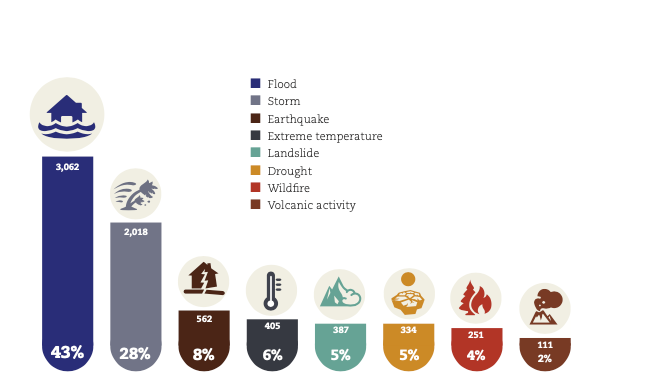
\includegraphics[scale=0.65]{img/stat1.png}
  \caption{Percentuale di eventi di calamità naturali per tipo di disastro  (1995-2015) \cite{2015human}.}
  \label{fig:floods}
\end{figure}
Le alluvioni sono tra le tipologie più gravi anche dal punto di vista dei danni economici, infatti, solo negli Stati Uniti si sono registrati 662 miliardi di dollari di danni causati da alluvioni (1995-2015) e nel continente europeo all’incirca 262 miliardi (1994-2015). Inoltre, le occorrenze di eventi disastrosi causati da fenomeni meteorologici risultano in crescita, in particolare, nel periodo tra il 2005 e il 2014 si è registrata una media di 335 eventi all’anno, ovvero il 14\% in più rispetto al periodo tra il 1995-2004 e quasi il doppio di quelli registrati tra il 1985 e il 1994. Lo stesso trend si può vedere nelle alluvioni, che nello stesso periodo (2005-2014) hanno raggiunto un picco di 171 eventi all’anno, rispetto ai 127 dei decenni precedenti \cite{2015human}.



\begin{figure}[h!]
    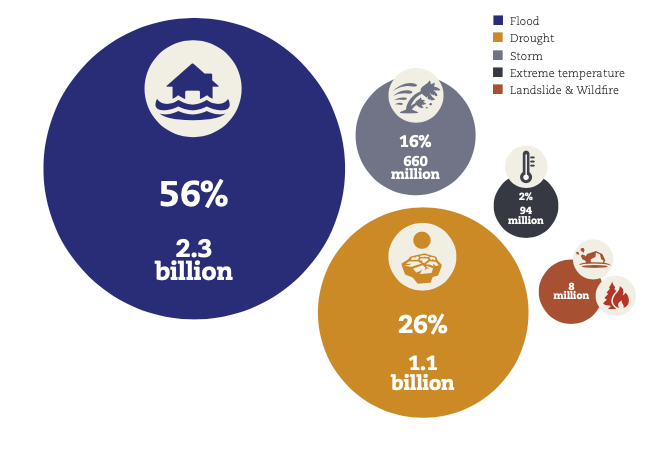
\includegraphics[scale=0.6]{img/stat2.png}
    \caption{Numero di persone colpite da calamità meteorologiche (1995-2015) (NB: i decessi sono esclusi dal totale delle vittime) \cite{2015human}.}
    \label{fig:flood_damage}
\end{figure}


In questo contesto, risulta essenziale la gestione di questi eventi disastrosi. In particolare, sono fondamentali le tre fasi di gestione delle alluvioni: la fase precedente all’evento, ovvero la fase di prevenzione; la fase durante l’evento stesso, in cui è fondamentale avere conoscenza sulle aree colpite e sul propagarsi dell’alluvione, informazioni che spesso non sono facili da reperire; e infine la fase post-alluvione, in cui si valutano i danni. Negli ultimi anni, nel campo della gestione dei disastri naturali, è risultato molto utile l’impiego di UAV (Unmanned Aerial Vehicle), anche chiamati droni. Uno dei primi utilizzi è stato nel 2005 negli Stati Uniti dove, per la prima volta, i droni sono stati utilizzati dal CRASAR (Center for Robot-Assisted Search and Rescue) dell’Università A\&M del Texas per cercare e soccorrere sopravvissuti agli eventi causati dall’Uragano Katrina. Successivamente, nel 2015, il CRASAR ha collaborato con la Measure UAV consulting firm e l’American Red Cross (ARC) per testare le capacità degli UAV in situazioni di emergenza ed eventi disastrosi, il report che ne seguì descrisse i droni come una tecnologia che portò “immediati benefici” sia ai civili che ai soccorritori. Fino ad oggi, i droni sono stati utilizzati in molti eventi di questo tipo, tra i tanti vi sono il terremoto di Wenchuan del 2008, la crisi di Fukushimi Daiichi del 2011 e la gestione del disastro causato dal Tifone Haiyan nelle Filippine nel 2013.
Infatti ad oggi, molte organizzazioni, principalmente umanitarie, hanno lanciato programmi che hanno come obiettivo quello di integrare gli UAV nelle operazioni di gestione di questi eventi, tra queste: l’WFP (ONU World Food Programme), la Banca Mondiale, l’UNHCR (UN High Commissioner for Refugees). In particolare, i droni hanno trovato utilità in tutte e tre le fasi menzionate precedentemente: nella fase di prevenzione vengono spesso utilizzati per monitorare il letto dei fiumi o altri bacini; durante le alluvioni vengono invece utilizzati per mappare le aree colpite, per operazioni di ricerca e soccorso, per il trasporto di carichi in zone altrimenti non raggiungibili, per fornire informazioni in tempo reale dall’alto sullo stato delle strade per guidare le squadre di soccorso, ma anche per fornire informazioni sugli edifici più colpiti per priorizzare le operazioni; infine, nel post-alluvione per la valutazione dei danni \cite{droneappl}.
%\section{Task}
%\label{section_task}
Uno dei principali vantaggi dei droni risiede nella rapidità del loro impiego e nell’alta risoluzione delle immagini che possono catturare. In particolare, con essi si riesce ad ottenere immagini di più alta risoluzione delle aree colpite ed in tempi più brevi rispetto ad altre risorse, come le immagini satellitari \cite{flyhurricane}. Inoltre, con l’elaborazione di queste immagini e grazie alla loro alta risoluzione, si riescono ad estrapolare informazioni molto importanti in questo ambito. Ad esempio, tra i vari utilizzi, si possono distinguere gli edifici e le strade allagate rispetto a quelle non allagate, si possono individuare alcuni oggetti di interesse quali persone o veicoli, oppure si può classificare il livello di danni di un edificio. Infatti, questo lavoro riguarda la segmentazione semantica, una delle tipologie di elaborazioni che spesso viene applicata alle immagini, per fornire informazioni molto utili soprattuto nella fase durante l'alluvione \cite{semsegsurvey}. La segmentazione semantica non è altro che la classificazione di ogni singolo pixel dell’immagine in una delle predeterminate classi (Figura \ref{fig:semseg})  e si distingue dal task della classificazione, in quanto quest’ultima riguarda l’assegnazione di una singola classe all’intera immagine. In particolare, il modello d’interesse di questo lavoro si occupa dell’assegnazione ad ogni pixel dell’immagine di una delle seguenti 9 classi: edificio allagato, edificio non allagato, strada allagata, strada non allagata, acqua, albero, veicolo e prato. Di queste, risultano di forte interesse nell'ambito della gestione di eventi di alluvione soprattutto le prime quattro classi, in quanto distinguere quali edifici siano allagati da quali no, può risultare fondamentale per guidare e priorizzare le operazioni di soccorso, mentre individuare le strade allagate può invece essere utile per distinguere quali strade siano percorribili via terra.

\begin{figure}[h!]
 \centering
 \begin{subfigure}[b]{0.45\textwidth}
     \centering
     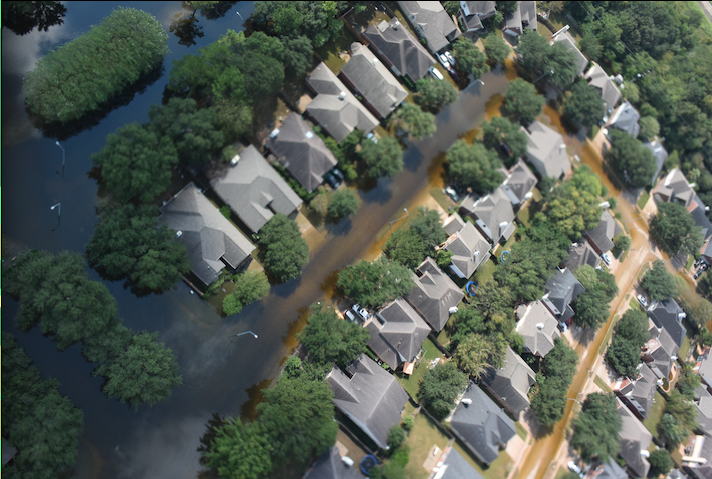
\includegraphics[width=\textwidth]{img/sem_seg copia 2.png}
     \caption{}
     \label{}
 \end{subfigure}
 \hfill
 \begin{subfigure}[b]{0.45\textwidth}
     \centering
     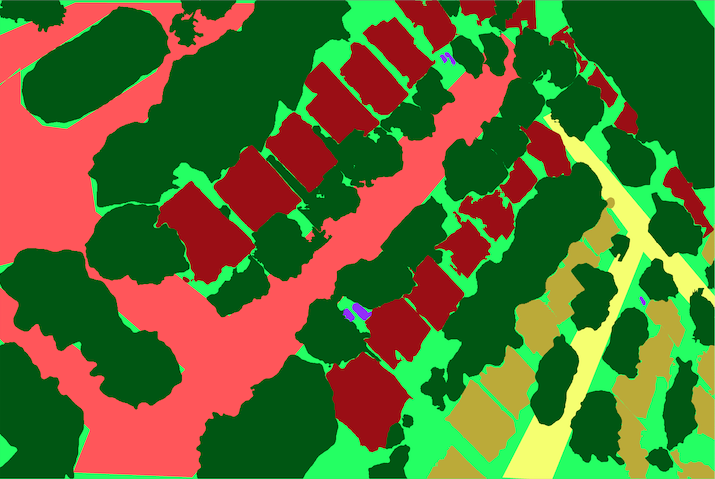
\includegraphics[width=\textwidth]{img/sem_seg copia.png}
     \caption{}
     \label{fig:bottleneck}
 \end{subfigure}
    \caption{Un esempio di segmentazione semantica. La (a) mostra l'immagine in input e la (b) l'output del modello, dove ogni colore corrisponde ad una classe: strada allagata (rosso chiaro), edificio allagato (rosso scuro), strada non allagata (giallo chiaro), edificio non allagato (giallo scuro), albero (verde scuro), prato (verde chiaro), veicolo (viola).}
    \label{fig:semseg}
\end{figure}
















\section{Stato dell'arte}
\label{stato_dell'arte}

Come vedremo più avanti, le reti neurali rispetto ai metodi più tradizionali riescono a cogliere informazioni di più alto livello. In particolare, la loro complessa architettura gli permette di approssimare pattern molto complessi, che i metodi tradizionali non riescono a cogliere. Infatti, come vedremo in questo paragrafo, nello stato dell'arte della segmentazione semantica di immagini aeree, la maggior parte delle metodologie utilizzate sono di Deep Learning.
Una delle architetture più presenti in letteratura e utilizzate in questo campo è la UNet. In diversi lavori \cite{safe_landing, uavid, kattenborn2019convolutional} viene utilizzata la versione classica proposta in \cite{unet}, in altri invece vengono utilizzate delle varianti. Ad esempio, in \cite{rescuenet} viene utilizzata la versione con l'aggiunta del meccanismo di attenzione, chiamata AttentionUnet \cite{attentionUnet}; in \cite{unet-segnet} viene utilizzata in combinazione con la SegNet \cite{segnet} per costruire un'architettura di tipo encoder-decoder (Figura \ref{fig:segnet-unet}); infine viene ripresa in \cite{real-time}, in cui viene utilizzata la rete MobileNet \cite{mobilenet} come backbone, ovvero come la prima parte della UNet (l'encoder) responsabile dell'estrazione delle feature. Ritornando invece su \cite{rescuenet}, il dataset RescueNet viene utilizzato come benchmark per diversi modelli tra cui, oltre all'AttentionUnet, la PSPNet \cite{pspnet}, la DeepLabV3+ \cite{deeplabv3+} e la ENet \cite{enet}. In altri lavori invece, vengono utilizzate architetture ensemble composte da più modelli. In particolare, in \cite{ensemble-cnns} un ensemble di CNN viene testato sul S-PRS Vaihingen Dataset. In questo caso l'ensemble è costituito da più versioni dello stesso modello, ovvero la stessa architettura addestrata più volte sullo stesso dataset  ma con inizializzazioni diverse. 


\begin{figure}[h!]
    \centering
    \hspace*{0in}
    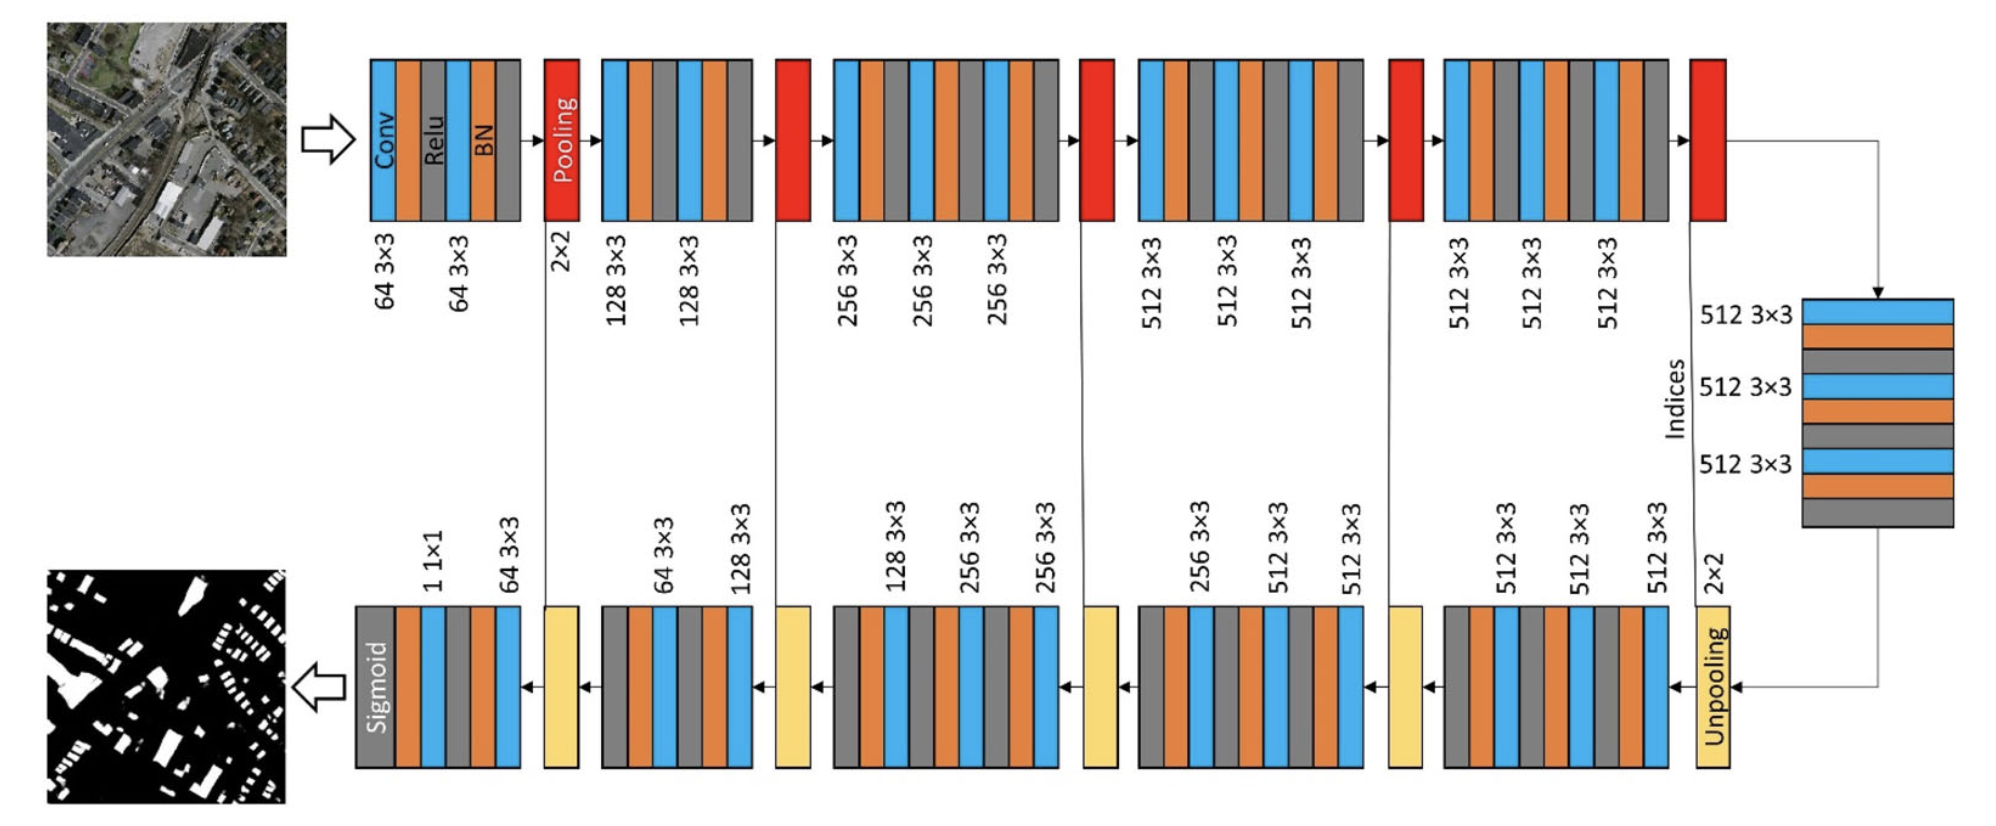
\includegraphics[scale=0.39]{img/segnet+unet.png}
    \caption{Architettura del modello Seg-Unet proposto in \cite{unet-segnet} con una combinazione dei componenti della Segnet (pooling indices) e quelli della Unet (skip connection).}
    \label{fig:segnet-unet}
\end{figure}


L'idea degli autori è che, essendo lo spazio della loss function in cui si muove il modello estremamente non convesso, a molte dimensioni e con molti minimi locali, inizializzare un modello con parametri diversi significa quasi avere la garanzia che convergerà in punti diversi. Di conseguenza, il loro approccio consiste nell'addestrare queste diverse versioni del modello per poi, in fase di inferenza, prendere la media delle loro predizioni. Un simile approccio viene utilizzato anche in \cite{shuffling-cnns}, in cui l'ensemble è composto dallo stesso modello ma preso in diverse fasi dell'addestramento. In particolare, gli autori evidenziano come, con questo approccio, sia possibile addestrare un ensemble senza aggiungere ulteriore tempo rispetto ad addestrare un singolo modello. Così come in \cite{rescuenet}, anche in \cite{hybrid-attention, luo2019high} vengono utilizzati modelli che si basano sul meccanismo di attenzione \cite{attention}. In particolare, gli autori  di \cite{hybrid-attention} evidenziano come un meccanismo  di attenzione ibrido, ovvero l'unione di diverse tipologie di attenzioni (sui canali, sullo spazio e sulle classi) riesca a catturare dipendenze a lungo raggio, aiutando così il modello a produrre delle feature map di qualità. Dall'altra parte, in \cite{luo2019high} gli autori, oltre a proporre un modello basato sulla struttura di una FCN con l'aggiunta del meccanismo di attenzione sui canali (\textit{channel attention mechanism}), propongono una approccio basato sull'utilizzo di due tipologie di dati corrisposte da due tipologie di backbone. In particolare, la prima parte del modello è composta da due ResNet101, una che prende in input l'immagine e una che invece prende in input dati ausiliari come l'NDVI (Normalized Difference Vegetation Index) ed altri. Nella seconda parte invece, le due feature map vengono concatenate e passate al modulo di \textit{channel attention}, per poi passare infine nella parte di upsample per produrre le maschere finali (Figura \ref{fig:channel_attention}).

\begin{figure}[h!]
    \centering
    \hspace*{0in}
    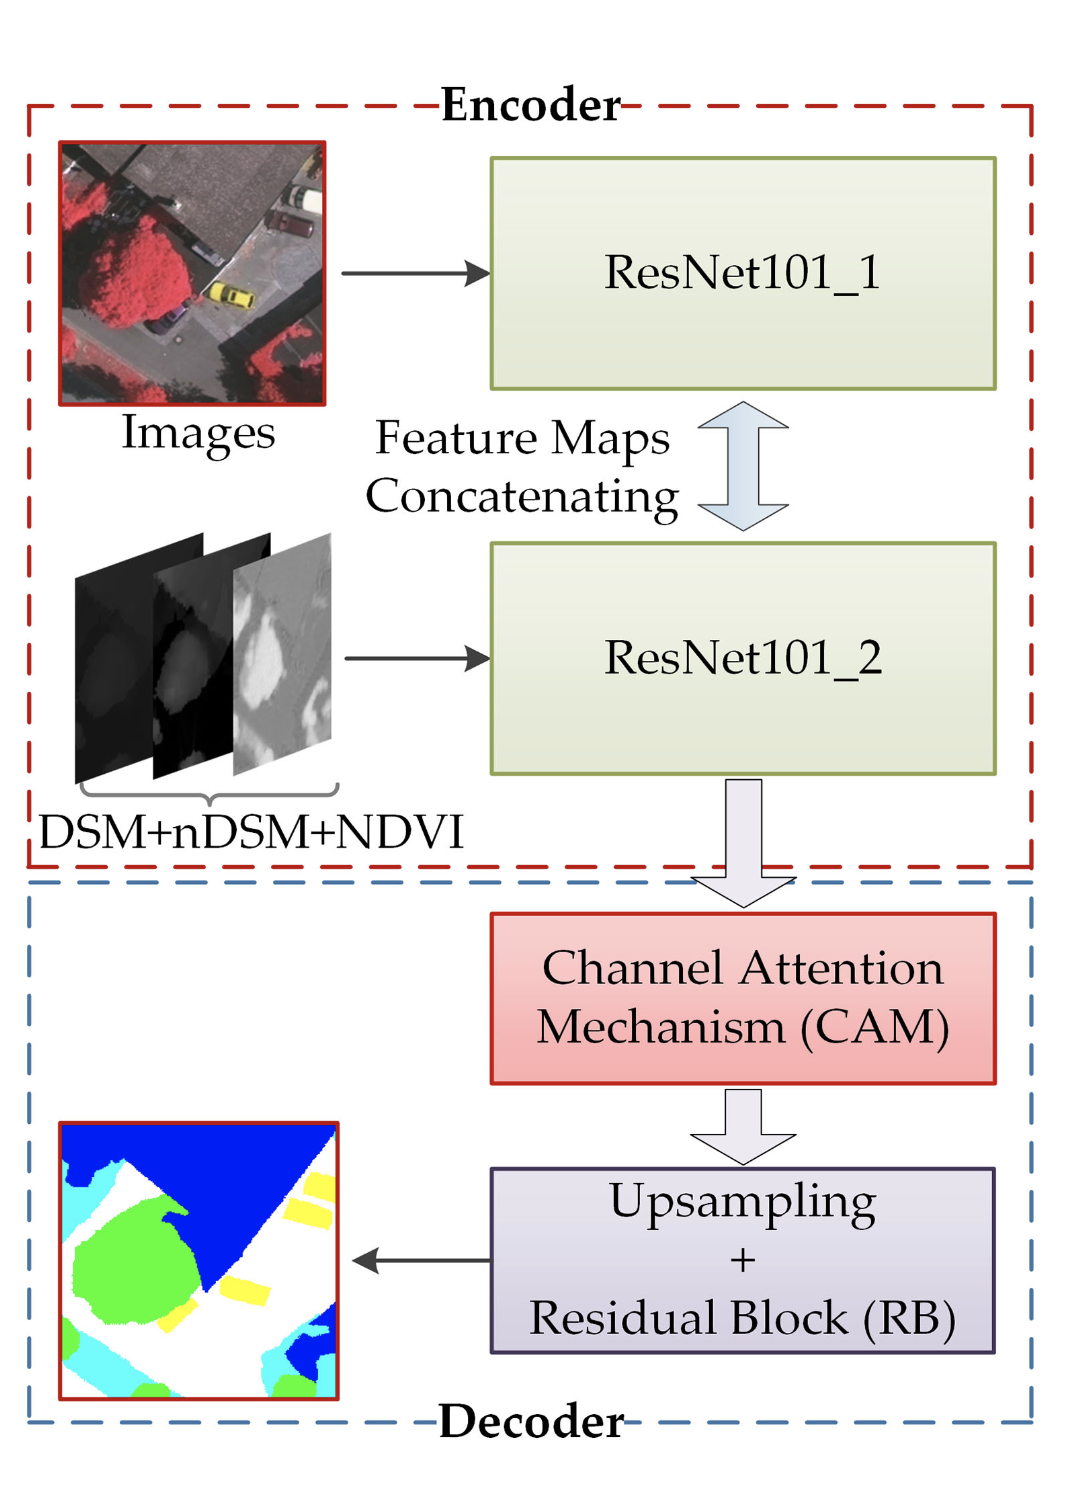
\includegraphics[scale=0.3]{img/chanel_attention_archi.png}
    \caption{Archittetura del modello basato sull'uso del \textit{channel attention mechanism} proposto in \cite{luo2019high}.}
    \label{fig:channel_attention}
\end{figure}





In \cite{distance_map} le maschere all'interno del dataset, prima di essere utilizzate per addestrare il loro modello, subiscono una prima fase di processing in cui vengono trasformate in delle \textit{distance maps}. In particolare, per ogni maschera e per ogni classe viene prodotta una maschera binaria, i cui valori dei pixel rappresentano la distanza di quel pixel di quella determinata classe dal bordo dell'oggetto di cui fa parte (Figura \ref{fig:distance_maps}).

\begin{figure}[h!]
    \centering
    \hspace*{-0.2in}
    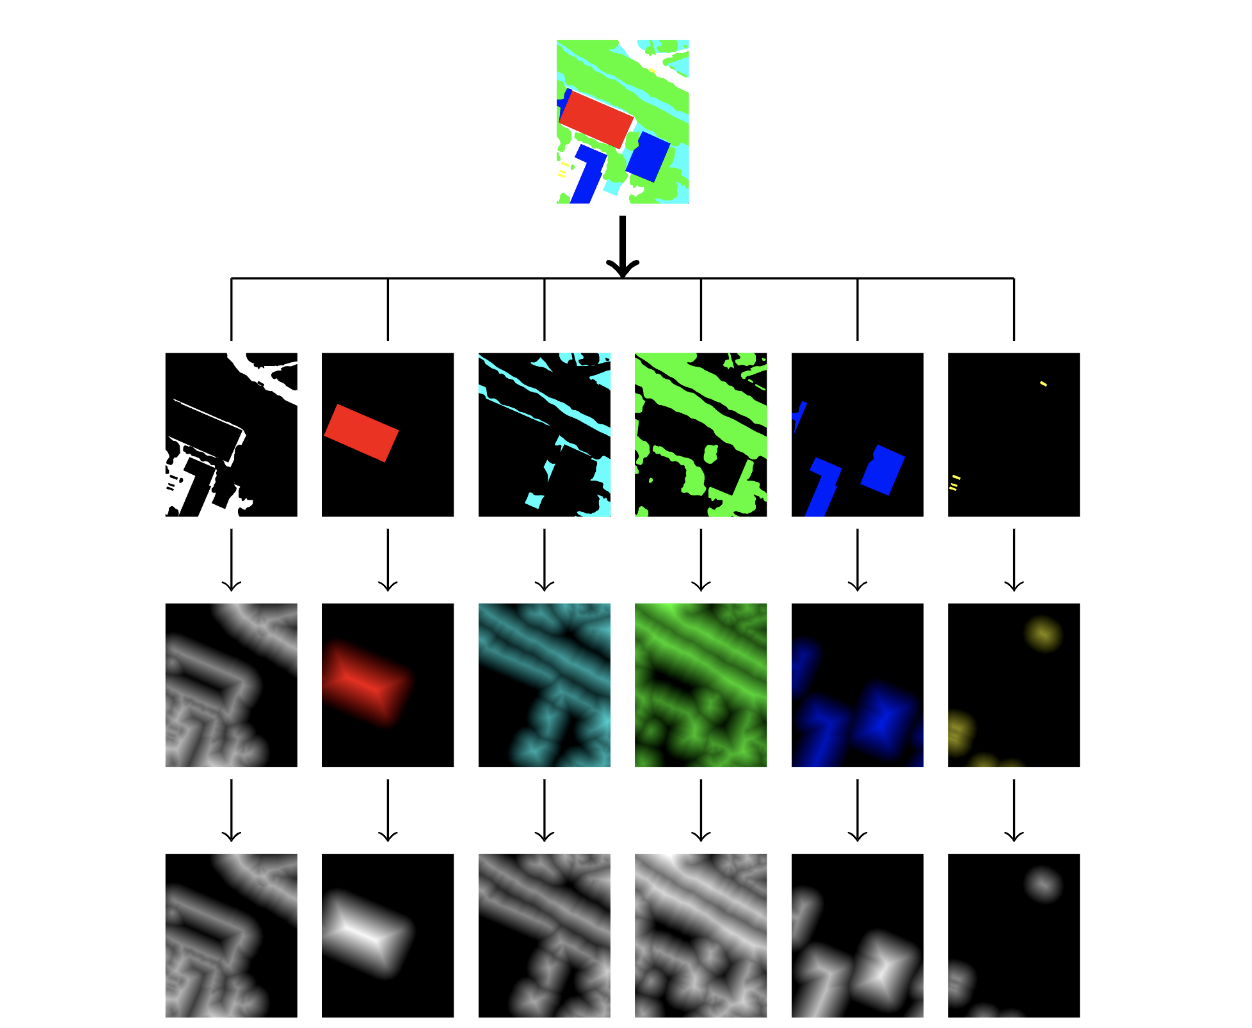
\includegraphics[scale=0.56]{img/distance_mps.png}
    \caption{Illustrazione della produzione di una \textit{distance map} a partire da una maschera \cite{distance_map}.}
    \label{fig:distance_maps}
\end{figure}

La motivazione per cui utilizzare le distance maps è che, grazie al fatto che codificano informazioni spaziali in più rispetto alle semplici maschere, gli output del modello ottenuto dal loro utilizzo nell'addestramento risultano con meno rumore, con più coerenza spaziale e i bordi degli oggetti appaiono più definiti (Figura \ref{fig:distance_map_result}).

\begin{figure}[h!]
     \centering
     \begin{subfigure}[b]{0.45\textwidth}
         \centering
         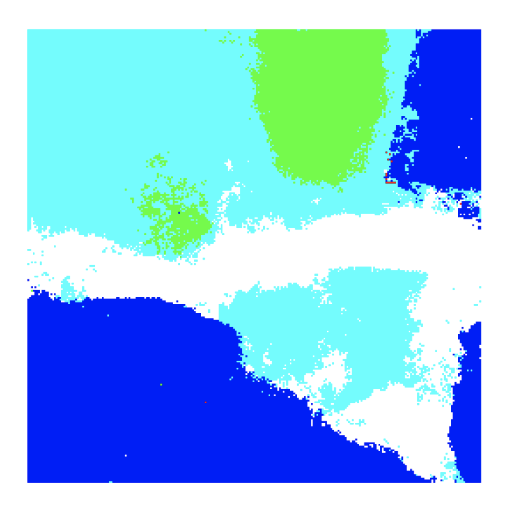
\includegraphics[width=\textwidth]{img/distance3.png}
         \caption{}
         \label{}
     \end{subfigure}
     \hfill
     \begin{subfigure}[b]{0.45\textwidth}
         \centering
         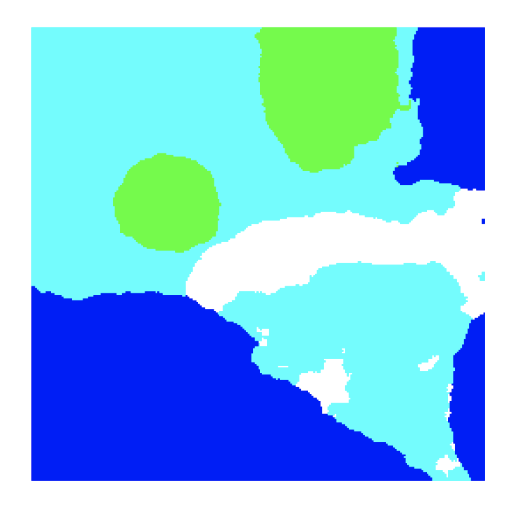
\includegraphics[width=\textwidth]{img/distance2.png}
         \caption{}
         \label{}
     \end{subfigure}
        \caption{La figura mostra il risultato del modello senza l'utilizzo delle \textit{distance maps} (a) e il risultato del loro utilizzo (b) \cite{distance_map}.}
        \label{fig:distance_map_result}
\end{figure}

Una variante della segmentazione semantica è quella affrontata in \cite{towards}, ovvero la segmentazione semantica open-set, che consiste nel task della segmentazione semantica, con l'aggiunta del fatto che il numero totale di classi è sconosciuto. Di conseguenza, la segmentazione semantica open-set può essere descritta come il task in cui ogni pixel può essere etichettato come appartenente a una delle classi apprese durante l'addestramento, oppure come una classe sconosciuta.
Le difficoltà di questa tipologia di task evidenziate dagli autori sono principalmente: la diversità di pattern nella classe sconosciuta e la similarità tra i pattern delle classi conosciute e quelli delle classi sconosciute. L'approccio proposto dagli autori consiste nel segmentare l'immagine con una CNN, che classifica pixel per pixel, e determinare una soglia per la quale se l'output della softmax della CNN non la supera, quel pixel viene classificato come classe sconosciuta. In aggiunta, propongono anche un ulteriore step per migliorare la qualità delle maschere prodotte e diminuire il numero di pixel della classe sconosciuta. In particolare, il metodo proposto, chiamato \textit{Morphological Filtering}, consiste nel riassegnare ogni pixel alla classe più presente nel suo vicinato e, nella pratica, l'effetto può essere visto come l'erosione della regioni classificate come classe sconosciuta (Figura \ref{fig:erosion}).

\begin{figure}[h!]
    \centering
    \hspace*{-0.17in}
    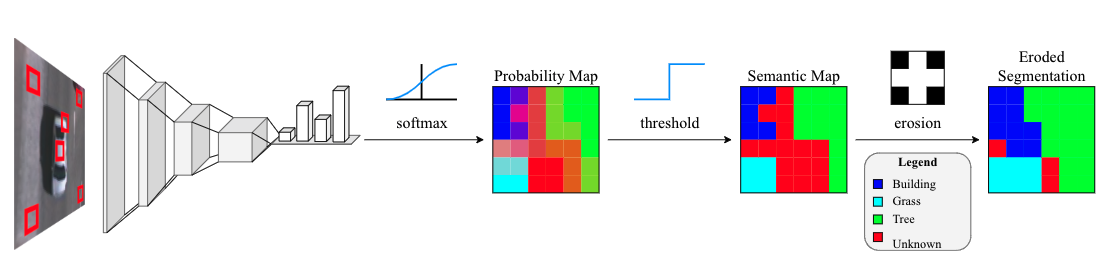
\includegraphics[scale=0.35]{img/erosion.png}
    \caption{Illustrazione del metodo proposto in \cite{towards}.}
    \label{fig:erosion}
\end{figure}




Altri lavori, come ad esempio \cite{three_dim}, utilizzano la segmentazione come step intermedio per altri task. In particolare, in quest'ultimo lavoro citato, le maschere prodotte vengono utilizzate per la stima della profondità delle acque di alluvioni e il modello utilizzato è una versione della FCN \cite{FCNs} con stride 8 (FCN-8s) e VGG-16 come backbone. In \cite{deep-based} vengono testate diverse versioni della UNet \cite{unet} e della LinkNet \cite{linknet}, combinando tra loro diversi modelli per la backbone e per la parte di decoder. Inoltre, gli autori hanno mostrato come in media su quasi tutti gli aspetti, i modelli che avevano la backbone pre addestrata su ImageNet abbiano performato meglio. In alcuni lavori invece, come \cite{sem_seg_ML}, oltre ad architetture di Deep Learning, vengono anche testati algoritmi di Machine Learning più tradizionali. Il loro lavoro riguarda il task della segmentazione delle diverse tipologie di vegetazione e, in particolare, il loro approccio è stato quello di testare diversi classificatori di ML, tra cui Random Forest, alberi decisionali e K-nearest neighbor. Per quanto riguarda, invece, l'architettura di Deep Learning da loro utilizzata, si tratta della SegNet \cite{segnet}. Infine, in \cite{floodnet} viene affrontato lo stesso specifico task di questo lavoro, ovvero il dataset FloodNet. In particolare, l'approccio degli autori consiste nel testare varie architetture, tra cui ENet \cite{enet}, PSPNet \cite{pspnet} e DeepLabV3+ \cite{deeplabv3+}. Nello specifico, gli autori evidenziano come le architetture che performano meglio siano quelle context-based e tra queste, la migliore è risultata la PSPNet.





















\section{Contributo ed Outline}
In questo lavoro viene esplorato il task della segmentazione semantica di immagini aeree del dataset FloodNet, attraverso approcci di Deep Learning. Nello specifico, viene proposto un nuovo approccio basato sulla risoluzione delle principali difficoltà individuate nel dataset. 
In particolare, il principale contributo di questo lavoro si può riassumere nei seguenti punti:


\begin{itemize}
    \item una fase di \textit{data cleaning}, per ovviare alla corposa presenza di errori nelle maschere del dataset.
    
    \item una fase di data augmentation offline, utile a far fronte ad un forte sbilanciamento del dataset verso alcune classi e alla presenza di altre in misura notevolmente minore.
    
    \item utilizzo di un'architettura context-based, mai utilizzata su questo dataset, volta ad ovviare alle difficoltà intrinseche di particolari classi, la cui semantica è fortemente basata sul loro contesto.
\end{itemize}

Per quanto riguarda la struttura dell'elaborato, esso è stutturato come segue. Nel Capitolo \ref{chapter_seg}, verrà esplorato il problema generale della segmentazione trattando le varie metodologie esistenti, sia tradizionali sia di Deep Learning. In seguito, nel Capitolo \ref{deep_learning}, si tratteranno i principali concetti di Deep Learning, approfondendo anche alcune delle architetture più note. Nel Capitolo \ref{chap_archi} invece, si entrerà nel dettaglio del task specifico di questo lavoro e si mostreranno, oltre all'architettura, anche le principali metodologie utilizzate.
Successivamente, nel Capitolo \ref{chap_exp} si illustreranno i vari esperimenti fatti durante tutto il lavoro e i loro risultati. Infine, nel Capitolo \ref{chap_conclusion} si trarranno le conclusioni del lavoro.